\documentclass[11pt,a4paper]{article}
\usepackage[margin=2.3cm]{geometry}
\usepackage{graphicx,booktabs,amsmath,siunitx,xcolor,tabularx,enumitem,listings}
\usepackage[version=4]{mhchem}
\usepackage[most]{tcolorbox}
\usepackage[hidelinks]{hyperref}
\graphicspath{{figures/}}
\setlist{itemsep=2pt,topsep=4pt}
\setlength{\parskip}{4pt}

\newtcolorbox{takeaway}{colback=blue!4,colframe=blue!50!black,boxrule=0.6pt,
  arc=2pt,left=6pt,right=6pt,top=4pt,bottom=4pt,fonttitle=\bfseries,title=Takeaway}
\newtcolorbox{pitfall}{colback=red!4,colframe=red!55!black,boxrule=0.6pt,
  arc=2pt,left=6pt,right=6pt,top=4pt,bottom=4pt,fonttitle=\bfseries,title=Pitfall}
\lstset{basicstyle=\ttfamily\small,columns=fullflexible,keepspaces=true,breaklines=true,
  aboveskip=3pt,belowskip=3pt}

\title{Learning notes: computational screening of photocatalysts\\[3pt]
\large Part I --- the project (organic photocatalysts) \quad Part II --- the DFT prework}
\author{Lindejiade}
\date{October 2026}

\begin{document}
\maketitle
\tableofcontents

%=============================================================================
\part*{Part I --- The project}
\addcontentsline{toc}{part}{Part I --- The project}

\section{Aim}

This project was suggested by my PI as a way to learn computational chemistry on a problem the lab
cares about. The idea is to take photocatalysts already reported in the literature and compute their
electronic structure: the energies and shapes of their frontier orbitals, and eventually their
excited states. Then I can see how far a standard DFT method gets in reproducing what experiment
measures. The plan has two halves. The first, covered here, is organic molecular photocatalysts,
computed with PySCF. The second will be solid-state photocatalysts such as \ce{TiO2}, using
Materials Project data and periodic DFT (Quantum ESPRESSO). Starting with molecules makes sense,
because every idea needed for solids (basis sets, functionals, orbital energies versus real gaps,
the effect of the environment) can be learned on systems small enough to run on a laptop.

\section{The 16 molecules and why they were chosen}

The catalogue contains 16 organic photocatalysts. It was assembled from standard reviews of organic
photoredox catalysis rather than by a formal screening procedure, but the final set satisfies
several criteria. First, it covers the main chromophore families: xanthene dyes (fluorescein,
eosin~Y, rose bengal, rhodamine~B), an acridinium (Mes-Acr$^+$), cyanoarenes (DCA, 4CzIPN), aryl
ketones and quinones (benzophenone, thioxanthone, benzil, anthraquinone), a phenothiazine (PTH), a
phenothiazinium dye (methylene blue), a flavin (riboflavin), a rylene diimide (Me-PDI) and a
porphyrin (TPP). Together they act through all the common mechanisms: an excited state that accepts
an electron (oxidative), one that donates an electron (reductive), energy transfer, singlet-oxygen
sensitisation, and hydrogen-atom transfer. Second, it includes landmark catalysts at the limits of
what organic photocatalysts can do: Mes-Acr$^+$ as a very strong excited-state oxidant, PTH as a
strong reductant, and 4CzIPN as a widely used, balanced catalyst. Third, a few molecules
(benzophenone, anthraquinone, eosin~Y) can abstract hydrogen atoms from C--H bonds, which connects
to the lab's methane work.

\begin{figure}[h]
\centering
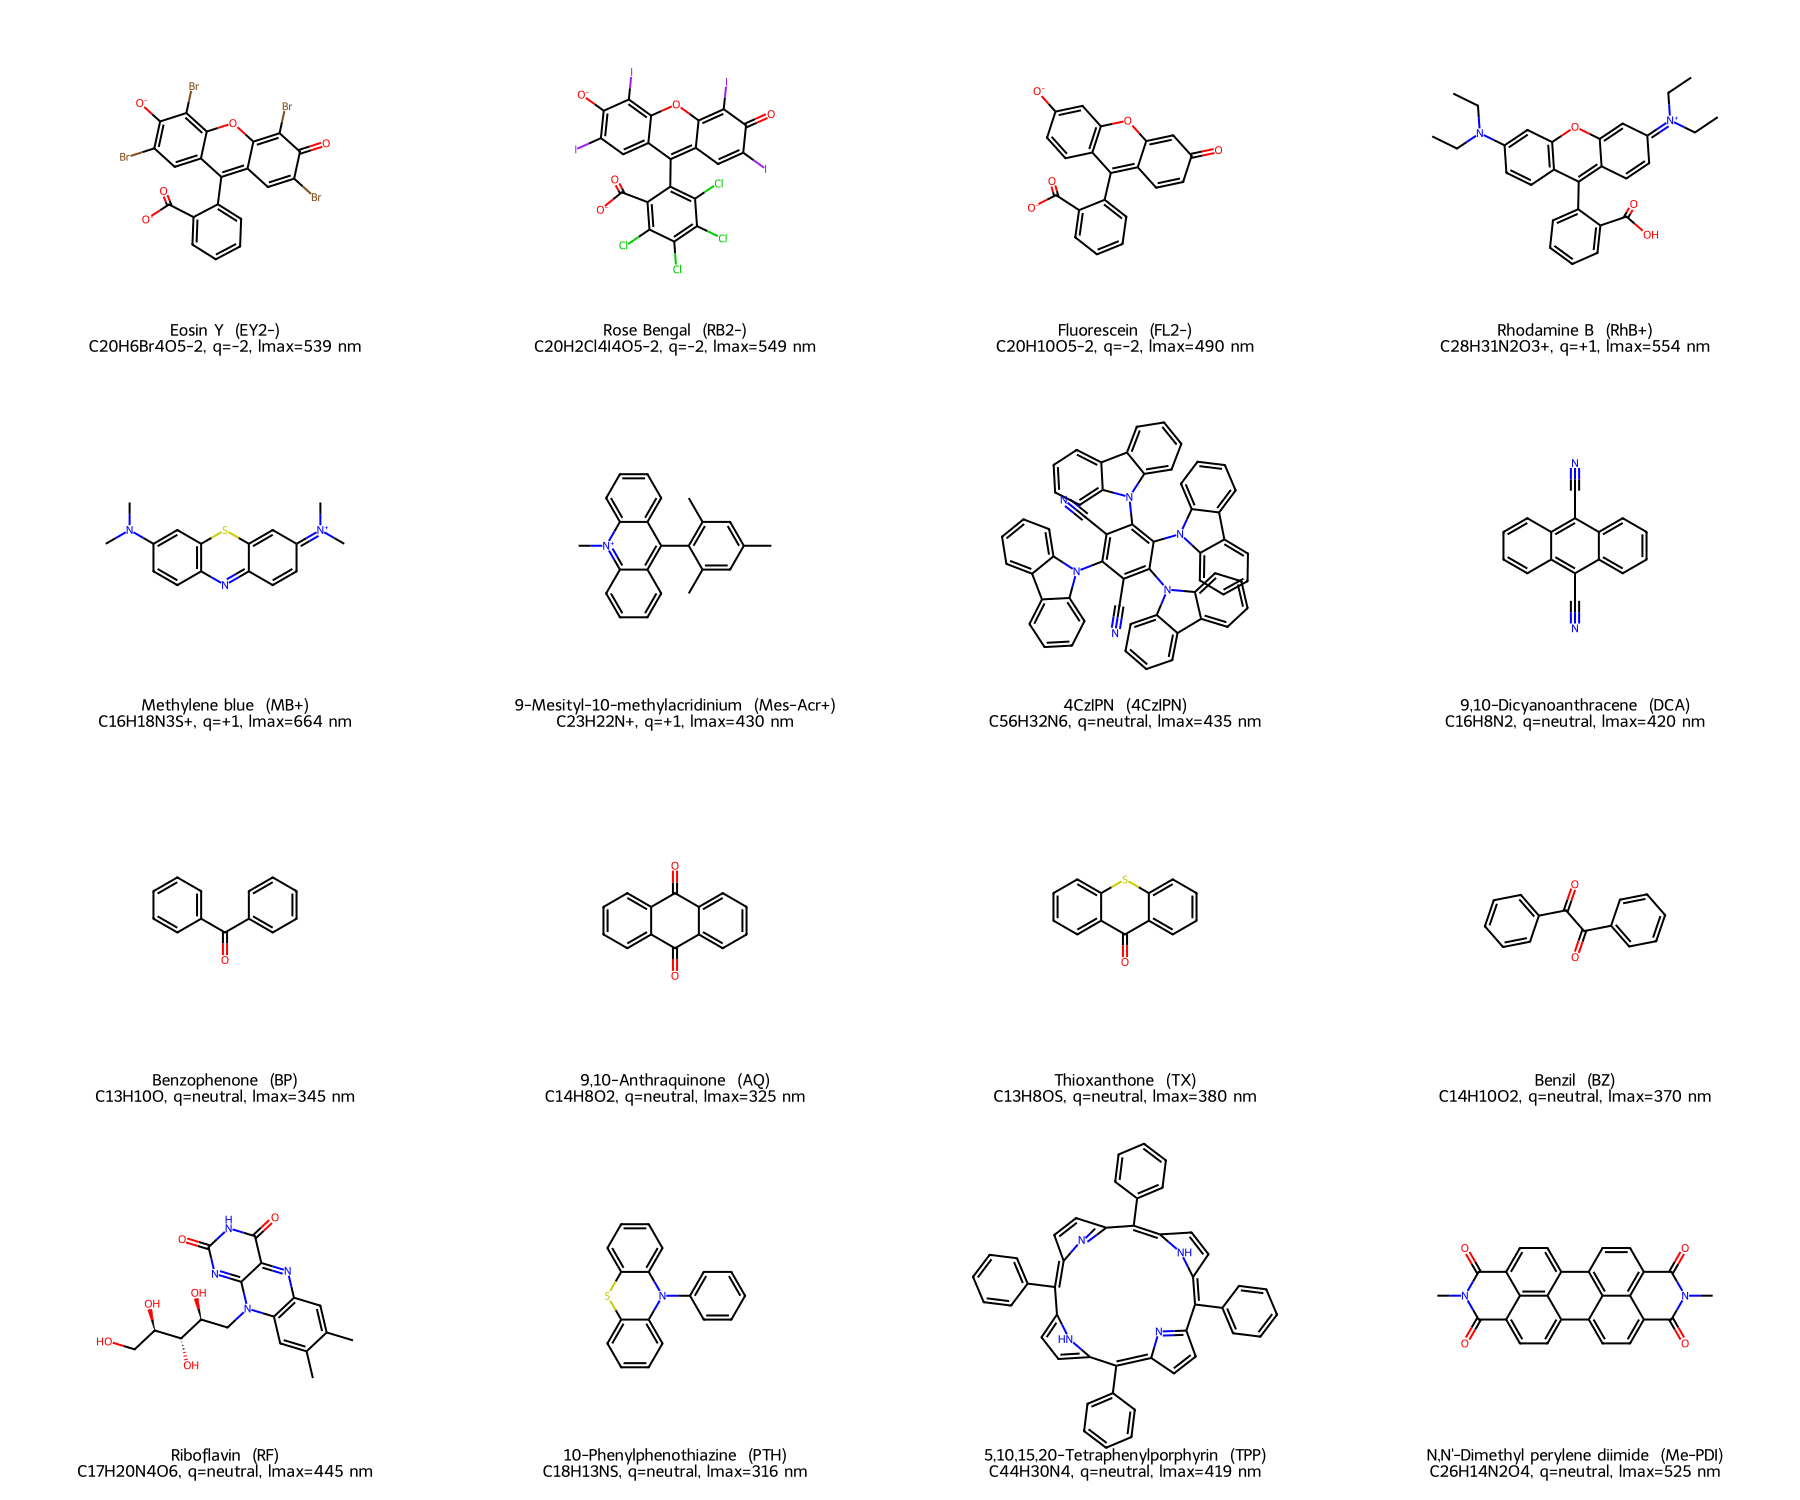
\includegraphics[width=0.8\linewidth]{organic_photocatalysts_grid.png}
\caption{The 16 molecules as encoded, each in its active charge state.}
\end{figure}

The most useful criterion for a learning project is that the set \emph{tests the method}. It contains
ions with charge $-2$ and $+1$, which need a solvent model; iodine, which needs an effective core
potential; three different kinds of excitation (local $\pi\to\pi^*$, n$\to\pi^*$ and charge
transfer); a clean substitution series on one skeleton (fluorescein $\to$ eosin~Y $\to$ rose bengal,
i.e.\ H $\to$ Br $\to$ I); rigid and flexible molecules; and sizes from 23 to 94 atoms. Every
molecule also has a measured absorption maximum to compare against. The set also has weak points.
The experimental spectra were measured in several different solvents. Rhodamine~B is better known
as a dye that gets degraded than as a catalyst. And only a few members are really relevant to C--H
activation; decatungstate, the clearest methane-activating photocatalyst, was postponed because it
is much more expensive to compute.

\section{How the calculations are set up}

The workflow has five steps, each a separate script. Step~1 turns each SMILES string into a checked
molecule and a 3D structure. Step~2 refines selected structures with a DFT geometry optimisation.
Step~3 computes the HOMO and LUMO energies of all 16 molecules. Step~4 draws the orbitals and
measures which part of each molecule they sit on. Step~5 checks whether using a force-field
geometry instead of a DFT one changes the orbital energies. Every calculation uses the same
\emph{level of theory}: the B3LYP functional, the def2-SVP basis set, and an implicit water
solvent (ddCOSMO, $\varepsilon = 78.36$). No dispersion correction is used, because the library
that provides it fails to load on my Mac.

Using water for \emph{every} molecule, neutral or charged, is a deliberate choice, and the main
reason is consistency. The whole project compares molecules with each other. If ions were computed
in water and neutral molecules in vacuum, every comparison between the two groups would mix a real
chemical difference with an artificial change of method. The solvent is essential for the ions: in
my prework (Lesson~5) it moved the HOMO of the phenolate anion by 4.5~eV. For a neutral, non-polar
molecule like anthraquinone it shifts the orbitals by only about 0.1~eV, so applying it everywhere
costs little. Two refinements matter, though. First, ``neutral'' does not mean ``unaffected''; what
the solvent responds to is the dipole. Anthraquinone's dipole is essentially zero, but riboflavin's
is 11.5~D, so riboflavin feels the solvent more. Second, water is a compromise, because the
experiments used different solvents. The solvent's effect scales roughly with
$(\varepsilon-1)/\varepsilon$, which is 0.99 for water and 0.97 for acetonitrile but only 0.79 for
chloroform. So treating every polar solvent as water is fine, but it is a real approximation for
the dyes measured in chloroform or dichloromethane.

\section{What has been found so far}

\paragraph{Geometries.} Six molecules have full DFT geometry optimisations. For the three rigid ones
(anthraquinone, thioxanthone, benzophenone) the force-field (MMFF) structure was already close to
DFT, within 0.02--0.10~\AA\ heavy-atom RMSD. For the three flexible or charged dyes (riboflavin,
eosin~Y$^{2-}$, rhodamine~B$^+$) it was not: they moved 0.17--0.40~\AA\ and dropped 11--20~kcal/mol
in energy. So the early conclusion that ``the force field is good enough'' was wrong for them.
Most of the movement is in carboxyl groups and side chains rather than in the light-absorbing
cores, so the orbital energies may change less than these numbers suggest. Step~5 was written to
test that, but it needs Step~3 to be rerun on the new geometries first.

\paragraph{Orbital energies.} Across the 16 dyes the B3LYP HOMO--LUMO gap correlates well with the
lowest experimental absorption band ($r = 0.90$). It is systematically too large (mean error
0.45~eV, larger than experiment for 13 of 16). This means the gap captures the \emph{trend} between
molecules, not the absorption energy itself. The first version of the energy-level diagram drew
the water-splitting redox levels across these orbital energies. That was misleading: B3LYP orbital
energies are not redox potentials. Those lines have now been removed.

\begin{figure}[h]
\centering
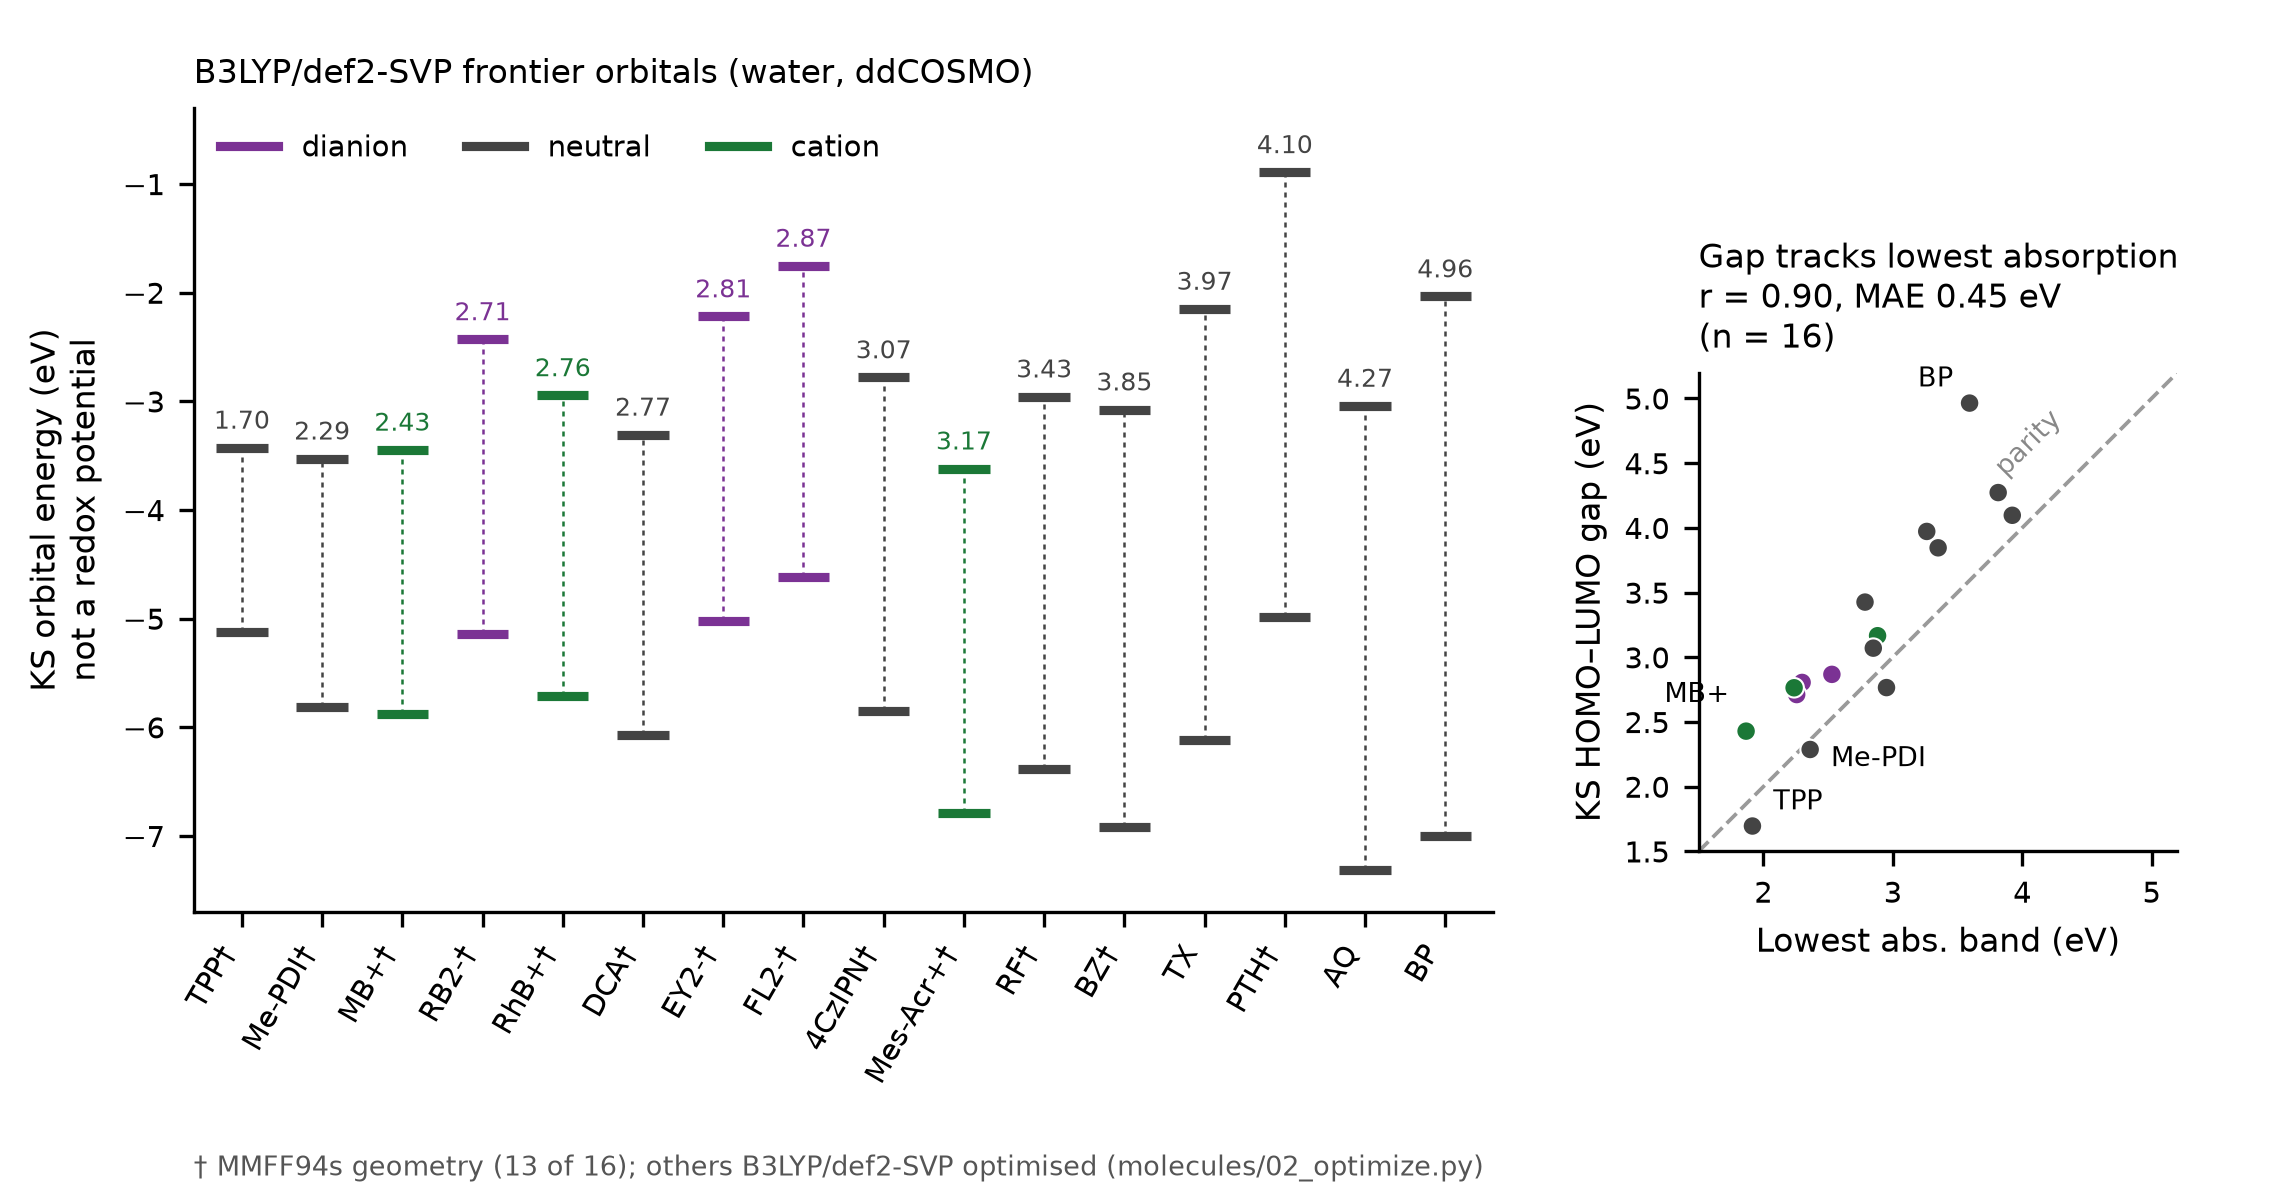
\includegraphics[width=0.95\linewidth]{homo_lumo_diagram.png}
\caption{B3LYP/def2-SVP frontier-orbital energies in water (left) and the gap against the lowest
experimental absorption band (right). Trend: good. Absolute values: not meaningful.}
\end{figure}

\paragraph{Where the orbitals live.} In eosin~Y$^{2-}$ the HOMO and LUMO are 91\% and 97\% on the
xanthene core. Its lowest excitation is therefore \emph{local}: the electron stays on the same part
of the molecule. In Mes-Acr$^+$ the LUMO is 98\% on the acridinium, while a donor orbital that is
96\% on the mesityl ring lies just below the HOMO. These two rings are held at 90$^\circ$ to each
other, which gives the molecule \emph{charge-transfer} character: an electron can be moved from
one ring to the other. This is the electronic origin of its strong oxidising power.

\paragraph{What is not done yet.} The project does not yet use TDDFT, so it has not actually
computed any absorption energies; the comparison above uses the HOMO--LUMO gap as a stand-in. Also
still to do: DFT geometries for the remaining ten molecules (depending on the Step~5 result), a
range-separated functional for the charge-transfer dyes, and all of the solid-state work.

%=============================================================================
\part*{Part II --- Skills needed, and the prework}
\addcontentsline{toc}{part}{Part II --- Skills needed, and the prework}

\section{Why I did the prework}

The repository grew faster than my understanding of it. Much of the code was written with AI
assistance (Claude and Claude Science), and it used ideas, such as multi-conformer searches,
Kabsch alignment and Mulliken fragment analysis, that I could not yet explain myself. Since the
purpose of the project is for me to learn DFT, I stepped back and worked through the basics on
small molecules first. The question I asked myself was what I need to understand to read this
project's code and results with confidence.

\section{How the prework was conducted}

The prework is six short lessons. Each uses one small molecule, about 20 lines of code, and
answers one question. All of them use the same level of theory as the project (B3LYP/def2-SVP in
PySCF), so the numbers are directly comparable. Lessons~3--5 were done in an exercise notebook
(\texttt{dft\_exercises\_L3-5.ipynb}). For each exercise I wrote the code myself, ran a
\emph{check} cell that compares my result with a known value, and answered a \emph{think}
question in my own words. Each calculation takes seconds to a few minutes on a laptop. The
principle throughout was to test on molecules whose answer I know (water, benzene) before trusting
the method on molecules whose answer I don't.

\begin{center}\small
\begin{tabularx}{\linewidth}{@{}clX@{}}
\toprule
& Lesson & Question \\
\midrule
1 & First DFT calculation (water) & What do the basis set and the functional each control? \\
2 & Geometry optimisation (water, benzene) & What do ``optimised'' and ``converged'' mean? \\
3 & Orbitals (benzene) & What do HOMO/LUMO energies mean, and what don't they mean? \\
4 & From SMILES (benzene, anthraquinone) & How does a string become a computable molecule? \\
5 & Charge and solvent (phenol, phenolate) & Why compute eosin~Y as $-2$, and in water? \\
6 & Back to the project (anthraquinone) & Can I reproduce a row of the project's results? \\
\bottomrule
\end{tabularx}
\end{center}

\section{What goes into a DFT calculation}

Before the lessons, one thing I had to get straight: what DFT actually takes as input. There are
two kinds. The first is the \emph{molecule}: which nuclei and where they are (elements and $x, y, z$
coordinates), the total charge, and the spin (the number of unpaired electrons). That is all the
physical information DFT receives. It is not told about bonds, SMILES or aromaticity; it works out
where the electrons go on its own, and the bonding follows from that. The second kind is the
\emph{method}: the functional (B3LYP), the basis set (def2-SVP), effective core potentials for
heavy atoms, the solvent model and numerical settings. Together these choices are called the
``level of theory''. In PySCF the two kinds map onto two lines:

\begin{lstlisting}
mol = gto.M(atom=atoms, charge=q, spin=0, basis="def2-svp")   # the molecule (+ basis)
mf  = dft.RKS(mol, xc="b3lyp")                               # the method
E   = mf.kernel()                                            # run the SCF; energy in Hartree
\end{lstlisting}

\noindent The output is the total energy, the orbitals (energies \texttt{mf.mo\_energy} and
coefficients \texttt{mf.mo\_coeff}) and the electron density. Geometry optimisation, TDDFT and
$\Delta$SCF all build on this one ground-state calculation.

\begin{pitfall}
PySCF can read an xyz file directly (\texttt{atom="eosinY.xyz"}), but it ignores the comment line,
which is where the project stores the charge. Read this way, eosin~Y came out as a neutral molecule
with 306 electrons instead of the dianion's 308, with no error or warning. That is why the project
parses the file itself (\texttt{read\_xyz}) and always passes \texttt{charge=} explicitly.
Coordinates come from the file; charge and spin must always be given separately.
\end{pitfall}

\section{The lessons}

\subsection*{Lesson 1 --- the first DFT calculation}
I ran water with three basis sets (STO-3G, def2-SVP, def2-TZVP) and three methods (Hartree--Fock,
PBE, B3LYP). A bigger basis always lowers the total energy: from STO-3G to def2-TZVP it drops by
1.1~Ha, about 3000~kJ/mol. Changing the functional moves it by about 0.4~Ha. So a total energy on
its own means nothing, and only differences computed at the \emph{same} level of theory are
meaningful. The orbital energies were even more revealing. Water's experimental ionisation energy
is 12.6~eV. Hartree--Fock's $-$HOMO gives 13.8~eV, but B3LYP's gives only 8.6~eV.

\subsection*{Lesson 2 --- geometry optimisation}
An optimisation repeats an SCF at fixed nuclei, which gives the energy and the force on each atom,
then moves the atoms downhill, until both the forces and the step sizes are below thresholds. For
water it gave O--H 0.967~\AA\ and an angle of 103.1$^\circ$ (experiment 0.958~\AA\ and
104.5$^\circ$). For benzene it gave C--C 1.398~\AA\ (experiment 1.397~\AA), in only 4 steps from a
force-field starting structure. A good starting geometry saves expensive DFT steps.

\subsection*{Lesson 3 --- orbitals, and what they don't mean}
Benzene has 42 electrons, so 21 occupied orbitals: the HOMO is orbital 20 (Python counts from 0).
Its HOMO and HOMO$-1$ have the same energy ($-6.97$~eV), and so do LUMO and LUMO$+1$ ($-0.25$~eV).
These are degenerate pairs, a consequence of the six-fold symmetry, so one member of a pair should
never be interpreted alone. The central result came from the ionisation energy:

\begin{center}\small
\begin{tabular}{@{}lr@{}}
\toprule
Method & Benzene IE (eV) \\
\midrule
Experiment & 9.24 \\
$-$HOMO, B3LYP & 6.97 \\
$-$HOMO, Hartree--Fock & 9.17 \\
$\Delta$SCF, B3LYP: $E(\ce{C6H6+}) - E(\ce{C6H6})$ & \textbf{9.24} \\
\bottomrule
\end{tabular}
\end{center}

B3LYP's $-$HOMO misses the ionisation energy by 2.3~eV because of \emph{self-interaction error}.
DFT computes the classical repulsion of the whole electron cloud, which includes each electron
repelling itself. Approximate functionals cancel only part of that. The leftover self-repulsion
pushes occupied orbital energies up, so electrons look less tightly bound than they are. The
$\Delta$SCF method avoids orbital energies entirely. It runs two complete calculations, the neutral
molecule and the cation, and subtracts the total energies. Most of the error cancels in the
subtraction, and the remaining electrons are allowed to relax after one is removed. Hartree--Fock
has no self-interaction; its $-$HOMO is close because two of its own errors (no relaxation, no
electron correlation) happen to cancel. The conclusion for the project: B3LYP orbital energies are
good for comparing molecules, not for absolute ionisation energies or redox potentials.

The orbitals were drawn with \texttt{cubegen}. This only turns the orbital's coefficients (114
numbers for benzene) into its values on a 3D grid, written to a cube file, so a viewer can draw
surfaces at $\pm$ an isovalue. It is a visualisation step and changes no results. The colours only
show the sign of the wavefunction; the nodes, where the sign changes, carry the physics.

\begin{figure}[h]
\centering
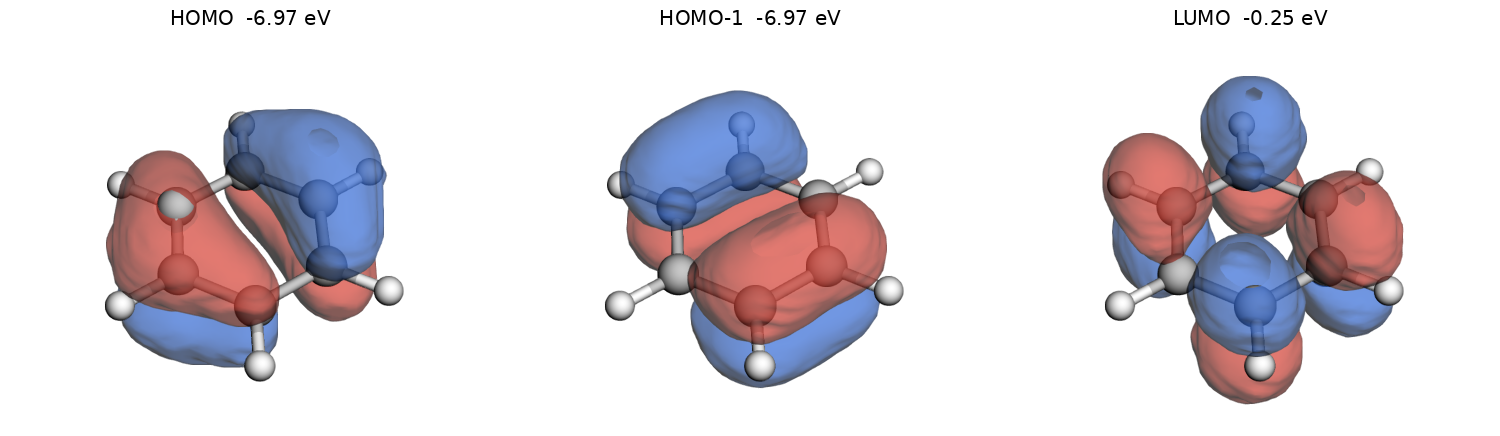
\includegraphics[width=0.75\linewidth]{benzene_frontier.png}
\caption{Benzene HOMO, HOMO$-1$ and LUMO ($\pm$0.03~a.u.). One nodal plane through the ring for
each HOMO, two for the LUMO: more nodes, higher energy.}
\end{figure}

Finally, \textbf{TDDFT}. Ground-state DFT only describes the lowest state, and the HOMO--LUMO gap
is not an absorption energy. When a molecule absorbs light, the excited electron and the hole it
leaves still attract each other, and a real excited state is usually a mixture of several orbital
jumps. TDDFT starts from the ground-state orbitals and asks at which frequencies of light the
electron density responds strongly, like the resonant frequencies of a guitar string. Each
resonance is an excited state, reported with an excitation energy and an \emph{oscillator
strength} $f$, which says how strongly that state absorbs light. For benzene, TDDFT puts S$_1$ at
5.48~eV with $f = 0$: symmetry-forbidden, which is why benzene's real 254~nm (4.9~eV) band is so
weak. It only appears at all because vibrations briefly break the symmetry. The strong band is
S$_3$/S$_4$ at 7.28~eV ($f = 0.59$), against about 6.9~eV measured. S$_1$ is three times closer to
experiment than the HOMO--LUMO gap (6.72~eV). This gives three distinct ``gaps'': the
\emph{KS gap} (6.72~eV, an orbital difference), the \emph{fundamental gap} (ionisation energy
minus electron affinity, about 10.4~eV) and the \emph{optical gap} (about 4.9~eV, the lowest
excitation). The optical gap is the smallest because the excited electron and hole stay on the
same molecule and attract each other. Photocatalysts act from their excited state, so TDDFT is
the tool the project still needs.

\subsection*{Lesson 4 --- from SMILES to a computable molecule}
\texttt{Chem.MolFromSmiles} returns an RDKit \texttt{Mol} object, a \emph{graph}. It knows each
atom's element, charge and aromaticity, how many hydrogens each atom carries, and which atoms are
bonded. It has no coordinates and no explicit hydrogen atoms. If the SMILES cannot be read, it
returns \texttt{None} \emph{without raising an error}, so this must always be checked. From the
graph to a calculation takes four steps: add explicit hydrogens, generate rough 3D coordinates
(ETKDG), clean them up with a force field (MMFF), and pass the list of (element, $x, y, z$) to
PySCF with the charge read from the SMILES:

\begin{lstlisting}
m  = Chem.MolFromSmiles(smiles);  q = Chem.GetFormalCharge(m)
mh = Chem.AddHs(m);  AllChem.EmbedMolecule(mh, params);  AllChem.MMFFOptimizeMolecule(mh)
pos   = mh.GetConformer().GetPositions()
atoms = [(a.GetSymbol(), tuple(pos[i])) for i, a in enumerate(mh.GetAtoms())]
mol   = gto.M(atom=atoms, basis="def2-svp", charge=q, spin=0)
\end{lstlisting}

\noindent For anthraquinone this gave a HOMO of $-7.288$~eV in water, against the project's
$-7.314$~eV. The 0.03~eV difference comes from the geometry, MMFF versus DFT-optimised. The
conformer search does not matter for such a rigid molecule, which has only one conformer. HOMO and
LUMO shift together, so the gap changed by only 0.007~eV. The solvent shifted the orbitals by only
about 0.1~eV, because anthraquinone is neutral and has almost no dipole.

\subsection*{Lesson 5 --- charge and solvent}
Phenol and phenolate are the smallest example of what happens at eosin~Y's phenol oxygen. Writing
\texttt{[O-]} in the SMILES removes a hydrogen and sets the charge to $-1$. When I built phenolate
without the charge, PySCF refused, because 49 electrons cannot all be paired. For a dianion,
however, losing the charge removes two electrons, the count stays even and nothing complains.
Then the results:

\begin{center}\small
\begin{tabular}{@{}lrrr@{}}
\toprule
& HOMO vacuum (eV) & HOMO water (eV) & Shift (eV) \\
\midrule
phenol (neutral) & $-6.18$ & $-6.26$ & $-0.08$ \\
phenolate ($-1$) & $+0.32$ & $-4.15$ & $-4.47$ \\
\bottomrule
\end{tabular}
\end{center}

In vacuum the anion's HOMO is \emph{positive}: the extra electron is not bound in this calculation.
Water stabilises it by 4.5~eV but the neutral molecule by only 0.08~eV, because the continuum
solvent responds to charge. Eosin~Y carries two such charges, which is why every ion in the project
is computed in water.

\subsection*{Lesson 6 --- back to the project}
Using only the route from Lesson~4, I ran a single point on the project's DFT-optimised
anthraquinone geometry in water. It reproduced the project's result to four decimal places (HOMO
$-7.3138$, LUMO $-3.0409$~eV). The project's Step~3 script is this same calculation in a loop over
16 molecules, plus bookkeeping. Reading the pipeline is now a matter of recognising these steps.

\section{Mistakes I made, and what they taught me}

Two of my own mistakes during the exercises taught me as much as the lessons did. First, my
$\Delta$SCF ionisation energy for benzene came out as 0.34. The value was right, but in Hartree:
PySCF returns energies in Hartree, and $0.34 \times 27.211 = 9.24$~eV. Total energies are large
(benzene is about $-232$~Ha), but the meaningful differences are small, so a suspiciously small
number usually means an unconverted unit. Useful conversions: 1~Ha = 27.211~eV = 627.5~kcal/mol =
2625.5~kJ/mol. Second, I used the SMILES for naphthalene instead of anthraquinone. Everything ran,
and the HOMO came out at $-5.97$~eV instead of about $-7.29$~eV. The giveaway was the electron
count: 68 instead of 108, and the run was suspiciously fast. A wrong SMILES is still a valid
SMILES, so the only protection is to check the result against something known independently, such
as the molecular formula. That is exactly why the project compares every SMILES with a stored
formula and charge.

\section{Key takeaways}

\begin{takeaway}
\begin{enumerate}[leftmargin=*]
  \item A DFT calculation needs only nuclei positions, charge and spin, plus the chosen
  functional, basis set and solvent. The charge must always be passed explicitly, and losing an
  even number of charges fails silently.
  \item Total energies are meaningless alone. Compare only differences, at the same level of
  theory, in the right units.
  \item B3LYP orbital energies are shifted by self-interaction error. They are good for trends
  between molecules, not for ionisation energies or redox potentials; $\Delta$SCF gives the real
  ionisation energy.
  \item The KS gap, the fundamental gap and the optical gap are different things. Absorption needs
  TDDFT, which also tells bright states from dark ones.
  \item SMILES $\to$ add H $\to$ ETKDG $\to$ MMFF $\to$ coordinates $\to$ PySCF is the whole route
  from a name to a calculation. Check the formula and the electron count before trusting it.
  \item Ions need a solvent model; non-polar neutral molecules barely notice it. Using one solvent
  for every molecule keeps comparisons fair.
  \item Test on molecules with known answers first. Every number in the project should be
  checked against something independent.
\end{enumerate}
\end{takeaway}

\section*{Questions for my PI}
\begin{itemize}
  \item Which functional does the group use for TDDFT on dyes, especially the charge-transfer
  ones?
  \item Should each molecule be computed in its experimental solvent rather than water?
  \item When is $\Delta$SCF in solvent preferred for redox potentials, and what corrections does it
  need?
  \item Should decatungstate move up the list, given its relevance to methane?
\end{itemize}

\end{document}
